\documentclass[a4paper,UTF8]{article}
\usepackage{amsmath}
\usepackage{amssymb}
\usepackage{amsthm}
\usepackage{bm}
\usepackage{color}
\usepackage{ctex}
\usepackage{enumerate}
\usepackage[margin=1.25in]{geometry}
\usepackage{graphicx}
\usepackage{hyperref}
\usepackage{tcolorbox}
\usepackage{algorithm}
\usepackage{algorithmic}
\usepackage{listings}
\theoremstyle{definition}
\newtheorem*{solution}{Solution}
\newtheorem*{prove}{Proof}
\newcommand{\indep}{\rotatebox[origin=c]{90}{$\models$}}
\usepackage{multirow}              

\setlength{\evensidemargin}{.25in}
\setlength{\textwidth}{6in}
\setlength{\topmargin}{-0.5in}
\setlength{\topmargin}{-0.5in}
% \setlength{\textheight}{9.5in}
%%%%%%%%%%%%%%%%%%此处用于设置页眉页脚%%%%%%%%%%%%%%%%%%
\usepackage{fancyhdr}                                
\usepackage{lastpage}                                           
\usepackage{layout}                                             
\footskip = 12pt 
\pagestyle{fancy}                    % 设置页眉                 
\lhead{2020年春季}                    
\chead{机器学习导论}                                                
% \rhead{第\thepage/\pageref{LastPage}页} 
\rhead{作业一}                                                                                               
\cfoot{\thepage}                                                
\renewcommand{\headrulewidth}{1pt}  			%页眉线宽,设为0可以去页眉线
\setlength{\skip\footins}{0.5cm}    			%脚注与正文的距离           
\renewcommand{\footrulewidth}{0pt}  			%页脚线宽,设为0可以去页脚线

\makeatletter 									%设置双线页眉                                        
\def\headrule{{\if@fancyplain\let\headrulewidth\plainheadrulewidth\fi%
		\hrule\@height 1.0pt \@width\headwidth\vskip1pt	%上面线为1pt粗  
		\hrule\@height 0.5pt\@width\headwidth  			%下面0.5pt粗            
		\vskip-2\headrulewidth\vskip-1pt}      			%两条线的距离1pt        
	\vspace{6mm}}     								%双线与下面正文之间的垂直间距              
\makeatother  


\begin{document}
\title{机器学习导论\\
	习题一}
\author{191300020, 黄彦骁, 191300020@smail.nju.edu.cn}
\maketitle


\section*{学术诚信}

本课程非常重视学术诚信规范,助教老师和助教同学将不遗余力地维护作业中的学术诚信规范的建立。希望所有选课学生能够对此予以重视。\footnote{参考尹一通老师\href{http://tcs.nju.edu.cn/wiki/}{高级算法课程}中对学术诚信的说明。}

\begin{tcolorbox}
	\begin{enumerate}
		\item[(1)] 允许同学之间的相互讨论,但是{\color{red}\textbf{署你名字的工作必须由你完成}},不允许直接照搬任何已有的材料,必须独立完成作业的书写过程;
		\item[(2)] 在完成作业过程中,对他人工作(出版物、互联网资料)中文本的直接照搬(包括原文的直接复制粘贴及语句的简单修改等)都将视为剽窃,剽窃者成绩将被取消。{\color{red}\textbf{对于完成作业中有关键作用的公开资料,应予以明显引用}};
		\item[(3)] 如果发现作业之间高度相似将被判定为互相抄袭行为,{\color{red}\textbf{抄袭和被抄袭双方的成绩都将被取消}}。因此请主动防止自己的作业被他人抄袭。
	\end{enumerate}
\end{tcolorbox}

\section*{作业提交注意事项}
\begin{tcolorbox}
	\begin{enumerate}
		\item[(1)] 请在\LaTeX模板中{\color{red}\textbf{第一页填写个人的姓名、学号、邮箱信息}};
		\item[(2)] 本次作业需提交该pdf文件、问题1,3可直接运行的源码(LinearRegression.py, PR.py, ROC.py,{\color{red}\textbf{不需要提交数据集}}),将以上三个文件压缩成zip文件后上传。zip文件格式为{\color{red}\textbf{学号.zip}},例如190000001.zip;pdf文件格式为{\color{red}\textbf{学号\_姓名.pdf}},例如190000001\_张三.pdf,{\color{red}\textbf{并通过教学立方提交}}。
		\item[(3)] 未按照要求提交作业,或提交作业格式不正确,将会{\color{red}\textbf{被扣除部分作业分数}};
		\item[(4)] 本次作业提交截止时间为{\color{red}\textbf{4月2日23:55:00。}}
	\end{enumerate}
\end{tcolorbox}

\newpage


\section{[45pts] Linear Regression with a Regularization Term}

给定数据集$D = \{(\mathbf{x}_1,y_1),(\mathbf{x}_2,y_2),\cdots,(\mathbf{x}_m,y_m)\}$, 其中$\mathbf{x}_i = (x_{i1};x_{i2};\cdots;x_{id}) \in \mathbb{R}^d$, $y_i \in \mathbb{R}$, 当我们采用线性回归模型求解时, 实际上是在求解下述优化问题:
\begin{equation}
	\label{eq:ls}
	\hat{\mathbf{w}}_{\textbf{LS}}^* = \mathop{\arg\min}_{\mathbf{w}} \frac{1}{2}\lVert  \mathbf {X}\mathbf{w}+\mathbf{1}\mathbf{b}^\top -\mathbf{y} \rVert_2^2\,,
\end{equation}
其中$\mathbf{y} = [y_1,\cdots,y_m]^\mathrm{T} \in \mathbb{R}^m, \mathbf{X} = [\mathbf{x}_1^\mathrm{T};\mathbf{x}_2^\mathrm{T};\cdots;\mathbf{x}_m^\mathrm{T}]\in \mathbb{R}^{m\times d}$, $\mathbf{1}$为全1向量,其维度可由其他元素推导而得。在实际问题中, 我们常常不会直接利用线性回归对数据进行拟合, 这是因为当样本特征很多, 而样本数相对较少时, 直接线性回归很容易陷入过拟合。为缓解过拟合问题, 常对公式\eqref{eq:ls}引入正则化项, 通常形式如下:

\begin{equation}
	\label{eq:ls-regular}
	\hat{\mathbf{w}}_{\textbf{reg}}^* = \mathop{\arg\min}_{\mathbf{w}} \frac{1}{2}\lVert \mathbf {X}\mathbf{w}+\mathbf{1}\mathbf{b}^\top -\mathbf{y} \rVert_2^2 +\lambda \Omega(\mathbf{w}),
\end{equation}
其中, $\lambda> 0$为正则化参数, $\Omega(\mathbf{w})$是正则化项, 根据模型偏好选择不同的$\Omega$。

下面, 假设样本特征矩阵$\mathbf{X}$满足列满秩, 请回答下面的问题:

(1) \textbf{[5pts]} 考虑线性回归问题, 即对应于公式\eqref{eq:ls}, 请给出最优解$\hat{\mathbf{w}}_{\textbf{LS}}^*$和$\mathbf{b}$的闭式解表达式,请使用矩阵形式表示;

(2) \textbf{[10pts]} 考虑{岭回归(ridge regression)}问题, 即对应于公式\eqref{eq:ls-regular}中$\Omega(\mathbf{w}) = \lVert \mathbf{w}\rVert_2^2$时, 请给出最优解$\hat{\mathbf{w}}_{\textbf{Ridge}}^*$和$\mathbf{b}$的闭式解表达式,请使用矩阵形式表示;

(3) \textbf{[15pts]} 请编程实现以上两种线性回归模型,基于你求出的闭式解在训练集上构建模型。并汇报测试集上的Mean Square Error (MSE)。

建议使用python语言实现,本次采用波士顿房价预测数据,数据集的获取依赖sklearn库,你可以查阅相关资料进行安装。请参考作业中提供的LinearRegression.py进行模型的构造,代码中已经完成了训练集和测试集的划分。
对于线性回归模型,你需要汇报测试集上的MSE,对于岭回归问题,你需要自行设置正则项$\lambda$的取值范围,并观察训练集MSE,测试集MSE和$\lambda$的取值的关系,你有什么发现?

请注意,除了示例代码中使用到的sklearn库函数以外,你将不能使用其他的sklearn函数,你需要基于numpy实现线性回归模型和MSE的计算。



(4) \textbf{[5pts]}如果推广到分类问题,应该如何设置$\mathbf{y}$,请谈谈你的看法;

(5) \textbf{[10pts]}请证明对于任何矩阵X,下式均成立
\begin{align}
	\left(\mathbf{X X}^{\top}+\lambda \mathbf{I}\right)^{-1} \mathbf{X}=\mathbf{X}\left(\mathbf{X}^{\top} \mathbf{X}+\lambda \mathbf{I}\right)^{-1}
\end{align}

请思考,上述的结论可以用在线性回归问题的什么情况中,能带来怎样的帮助?

提示1:你可以参考 \href{https://www.math.uwaterloo.ca/~hwolkowi/matrixcookbook.pdf}{The Matrix Cookbook}获取矩阵求导的一些知识。

\begin{solution}
	\begin{enumerate}
		\item[(1)] 令$\beta=\left\{\mathbf{w}; \mathbf{b}^{\top}\right\},\mathbf{X_1}=\left\{\mathbf{X};\mathbf{1}\right\}$,
		      则方程转化为$\frac{1}{2}\lVert \mathbf{X_1}\beta-\mathbf{y} \rVert_2^2 $,则通过对其求梯度为0可得$\beta=(\mathbf{X_1}^{\top}\mathbf{X_1})^{-1}\mathbf{X_1}^{\top}\mathbf{y}$,
		      则可以得到$\hat{\mathbf{w}}_{\textbf{LS}}^* = \mathbf{A}\beta,\mathbf{b} = \mathbf{B}\beta$,其中:
		      \[A = \begin{bmatrix}
				      1      & 0      & 0      & \cdots & 0      & 0      \\
				      0      & 1      & 0      & \cdots & 0      & 0      \\
				      \vdots & \vdots & \vdots &        & \vdots & \vdots \\
				      0      & 0      & 0      & \cdots & 1      & 0
			      \end{bmatrix}_{d * (d+1)}\]
		      \[B=\begin{bmatrix}
				      0 & 0 & 0 & \cdots & 0 & 1
			      \end{bmatrix}_{1*(d+1)}\]
		\item[(2)]
		      将方程对$\mathbf{w}$和$\mathbf{b}$分别求偏导得:
		      \[\frac{\partial{E}}{\partial{\mathbf{w}}} = \mathbf{X}^{\top}(\mathbf{X}\mathbf{w}+1\mathbf{b}^{\top}-\mathbf{y})+2\lambda \mathbf{w}\]
		      \[\frac{\partial{E}}{\partial{b}}=(\mathbf{X}\mathbf{w}+1\mathbf{b}^{\top}-\mathbf{y})^{\top}·1\]
		      得到
		      \[\hat{w}^*_{Ridge}=(m(\mathbf{X}^{\top}\mathbf{X}+2\lambda \mathbf{I})-\mathbf{X}^{\top}1·1^{\top}\mathbf{X})^{-1}(m\mathbf{X}^{\top}\mathbf{y}-\mathbf{X}^{\top}1·1^{\top}\mathbf{y})\]
		      \[\hat{b^T}=\frac{1}{m}(1^{\top}\mathbf{y}-1^{\top}\mathbf{X}\hat{\mathbf{w}}^*_{Ridge})\]
		\item[(3)]当$\lambda$逐渐增大时,$MSE$逐渐变大
		\item[(4)]
		      若属性值间存在“序”关系,可通过连续化将其转化为连续值,否则转化为多维向量。
		\item[(5)]
		      将题中等式化简有:
		      \begin{align*}
			                      & \left(\mathbf{X X}^{\top}+\lambda \mathbf{I}\right)^{-1} \mathbf{X}=\mathbf{X}\left(\mathbf{X}^{\top} \mathbf{X}+\lambda \mathbf{I}\right)^{-1} \\
			      \Leftrightarrow & \mathbf{X}(\mathbf{X}^{\top}\mathbf{X}+\lambda\mathbf{I})=(\mathbf{X}\mathbf{X}^{\top}+\lambda\mathbf{I})\mathbf{X}                             \\
			      \Leftrightarrow & \mathbf{X}\mathbf{X}^{\top}\mathbf{X}+\lambda\mathbf{X}\mathbf{I} =\mathbf{X}\mathbf{X}^{\top}\mathbf{X}+\lambda\mathbf{I}\mathbf{X}            \\
			      \Leftrightarrow & \lambda\mathbf{X}\mathbf{I}=\lambda\mathbf{I}\mathbf{X}
		      \end{align*}
		      由于$\mathbf{I}$为单位矩阵,所以显然有$\mathbf{X}\mathbf{I}=\mathbf{I}\mathbf{X}$,故题中等式成立。\\
		      思考:对岭回归有帮助,可以简化计算。
	\end{enumerate}

\end{solution}

\section{[25+5pts] Multi-Class Logistic Regression}
教材的章节3.3介绍了对数几率回归解决二分类问题的具体做法。假定现在的任务不再是二分类问题,而是多分类问题,其中$y\in\{1,2\dots,K\}$。请将对数几率回归算法拓展到该多分类问题。


(1) \textbf{[15pts]} 给出该对率回归模型的“对数似然”(log-likelihood);

(2) \textbf{[10pts]} 请仿照课本公式3.30,计算该“对数似然”的梯度;

(3) \textbf{[Bonus 5pts]} 对于样本类别分布不平衡的问题,基于以上的推导会出现怎样的问题,应该进行怎样的应对?谈谈你的看法。


提示1:假设该多分类问题满足如下$K-1$个对数几率,
\begin{eqnarray*}
	\ln\frac{p(y=1|\mathbf{x})}{p(y=K|\mathbf{x})}&=&\mathbf{w}_1^\mathrm{T}\mathbf{x}+b_1\\
	\ln\frac{p(y=2|\mathbf{x})}{p(y=K|\mathbf{x})}&=&\mathbf{w}_2^\mathrm{T}\mathbf{x}+b_2\\
	&\dots&\\
	\ln\frac{p(y={K-1}|\mathbf{x})}{p(y=K|\mathbf{x})}&=&\mathbf{w}_{K-1}^\mathrm{T}\mathbf{x}+b_{K-1}
\end{eqnarray*}

提示2:定义指示函数$\mathbb{I}(\cdot)$,
$$\mathbb{I}(y=j)=
	\begin{cases}
		1 & \text{若$y$等于$j$}   \\
		0 & \text{若$y$不等于$j$}
	\end{cases}$$

\begin{solution}
	\begin{enumerate}
		\item [(1)] 由满足的对数几率可以求得:
		      \[p\left[ y=i |\mathbf{x}\right] = \frac{e^{\mathbf{w}_i^\mathrm{T}\mathbf{x}+b_i}}{1+\sum_{j=1}^{K-1}e^{\mathbf{w}_j^\mathrm{T}\mathbf{x}+b_j}},i=1\ldots K-1\]
		      \[p\left[y=K | \mathbf{x}\right] = \frac{1}{1+\sum_{j=1}^{K-1}e^{\mathbf{w}_j^\mathrm{T}\mathbf{x}+b_j}}\]
		      令$\beta_i = (\mathbf{w}_i;b_i), \hat{\mathbf{x}}=(\mathbf{x};1)$,则$\mathbf{w}_i^\mathrm{T}\mathbf{x}+b_i=\beta_i^\mathrm{T}\hat{\mathbf{x}}$
		      则似然项可以写为:
		      \[p(y_i|\mathbf{x}_i;\mathbf{w},b)=\sum_{j=1}^{K}\mathbb{I}(y_i=j)p(y_i=j|\hat{\mathbf{x_i}};\beta_i)\]
		      求得对数似然项为:
		      \[l(\beta) = \sum_{i=1}^m(\sum_{j=1}^{K-1}\mathbb{I}(y_i=j)\beta_j^\mathrm{T}\hat{\mathbf{x_i}}-ln(1+\sum_{j=1}^{K-1}e^{\beta_j^\mathrm{T}\hat{\mathbf{x_i}}}))\]

		\item [(2)]对对数似然求梯度得:
		      \[\frac{\partial{l}}{\partial{\beta}} = (\sum_{i=1}^m\hat{\mathbf{x_i}}(\mathbb{I}(y_i=1)-p(y_i = 1|\hat{\mathbf{x_i}})), \ldots, \sum_{i=1}^m\hat{\mathbf{x_i}}(\mathbb{I}(y_i=K-1)-p(y_i = K-1|\hat{\mathbf{x_i}})))_{1*(K-1)}\]
		\item [(3)] 不会产生影响。
	\end{enumerate}
\end{solution}


\section{[30pts] P-R Curve \& ROC Curve}
现有500个测试样例,其对应的真实标记和学习器的输出值如表\ref{table:roc}所示 (完整数据见data.csv文件)。该任务是一个二分类任务,1表示正例,0表示负例。学习器的输出越接近1表明学习器认为该样例越可能是正例,越接近0表明学习器认为该样例越可能是负例。
\begin{table}[!h]
	\centering
	\caption{测试样例表} \vspace{2mm}\label{table:roc}
	\begin{tabular}{c|c c c c c c c c c c c}\hline
		样本   & $x_1$ & $x_2$ & $x_3$ & $x_4$ & $x_5$ & ... & $x_{496}$ & $x_{497}$ & $x_{498}$ & $x_{499}$ & $x_{500}$ \\
		\hline
		标记   & 1     & 1     & 0     & 0     & 0     & ... & 0         & 1         & 0         & 1         & 1         \\
		\hline
		输出值 & 0.206 & 0.662 & 0.219 & 0.126 & 0.450 & ... & 0.184     & 0.505     & 0.445     & 0.994     & 0.602     \\
		\hline
	\end{tabular}
\end{table}

(1) \textbf{[10pts]}请编程绘制P-R曲线;

(2) \textbf{[15pts]}请编程绘制ROC曲线,并计算AUC;

(3)	 \textbf{[5pts]} 需结合关键代码说明思路,并附最终绘制的曲线。建议使用python编程实现。
实验报告需要有层次和条理性,能让读者仅通过实验报告便能了解实验的目的,过程和结果。



提示1: 需要注意数据中存在输出值相同的样例。

提示2: 在python中,数值计算通常使用numpy, 表格数据操作通常使用pandas, 画图可以使用matplotlib, 可以通过上网查找相关资料学习使用这些工具。未来大家会接触到更多的python扩展库,如集成了众多机器学习方法的sklearn, 深度学习工具包pytorch等。

\begin{solution}
	\begin{enumerate}
		\item [(3)]
		      \begin{lstlisting}
import numpy as np
import pandas as pd
import matplotlib.pyplot as plt

data = pd.read_csv("data.csv", index_col=0)
data = data.sort_values('output', ascending=False)
target = data['output'].unique()
n = len(target)
for i in range(n):
	data['prediction'] = data['output'] >= target[i]
	TP = np.sum((data['label'] == 1) & (data['prediction'] == 1))
	FP = np.sum((data['label'] == 0) & (data['prediction'] == 1))
	TN = np.sum((data['label'] == 0) & (data['prediction'] == 0))
	FN = np.sum((data['label'] == 1) & (data['prediction'] == 0))
	\end{lstlisting}
		      将数据中的$"output"$进行去重并从大到小排序存入$target$中,然后循环取$target$中得值来作为划分,分别计算$TP,FP,TN,FN$存好
		      \begin{lstlisting}
P[i] = TP / (TP + FP)
R[i] = TP / (TP + FN)
TPR[i] = TP / (TP + FN)
FPR[i] = FP / (FP + TN)
		\end{lstlisting}
		      然后在$for$循环中按照公式计算$P,R$或者$TPR,FPR$,最后绘图:
		      \begin{figure}[h]
			      \centering
			      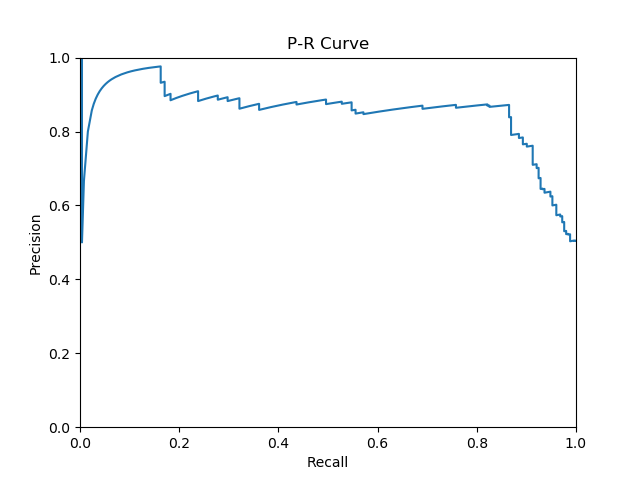
\includegraphics[width=8cm,height=6cm]{PR.png}
			      \caption{PR-曲线}
		      \end{figure}
		      \begin{figure}[h]
			      \centering
			      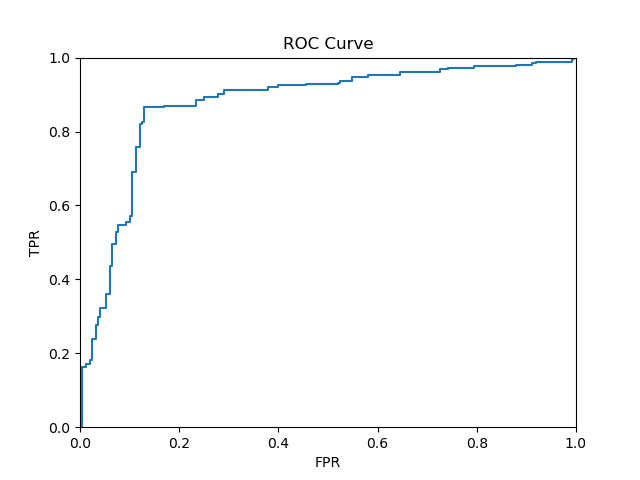
\includegraphics[width=8cm,height=6cm]{ROC.png}
			      \caption{ROC-曲线}
		      \end{figure}
		      $AUC$由公式$AUC = np.sum((FPR[1:] - FPR[:-1]) * (TPR[:-1] + TPR[1:])) / 2$计算得为0.8737
	\end{enumerate}
\end{solution}

\end{document}